\documentclass[12pt,a4paper]{report}

\usepackage[utf8]{inputenc} % pentru suport diacritice
\usepackage[romanian]{babel} % setări pentru limba română 
\renewcommand\familydefault{\sfdefault} % sans serif

\usepackage[margin=2.54cm]{geometry}	% dimensiuni pagină și margini
\usepackage{graphicx} % support the \includegraphics command and options

% formatting sections and subsections
\usepackage{textcase}
\usepackage[titletoc, title]{appendix}
\usepackage{titlesec}
\titleformat{\chapter}{\large\bfseries\MakeUppercase}{\thechapter}{2ex}{}[\vspace*{-1.5cm}]
\titleformat*{\section}{\large\bfseries}
\titleformat*{\subsection}{\large\bfseries}
\titleformat*{\subsubsection}{\large\bfseries}

\usepackage{chngcntr}
\counterwithout{figure}{chapter} % no chapter number in figure labels
\counterwithout{table}{chapter} % no chapter number in table labels
\counterwithout{equation}{chapter} % no chapter number in equation labels

\usepackage{booktabs} % for much better looking tables
\usepackage{url} % Useful for inserting web links nicely
\usepackage[bookmarks,unicode,hidelinks]{hyperref}

\usepackage{array} % for better arrays (eg matrices) in maths
\usepackage{paralist} % very flexible & customisable lists (eg. enumerate/itemize, etc.)
\usepackage{verbatim} % adds environment for commenting out blocks of text & for better verbatim
\usepackage{subfig} % make it possible to include more than one captioned figure/table in a single float
\usepackage{enumitem}
\setlist{noitemsep}

%%% HEADERS & FOOTERS
\usepackage{fancyhdr}
\pagestyle{empty}
\renewcommand{\headrulewidth}{0pt}
\renewcommand{\footrulewidth}{0pt}
\lhead{}\chead{}\rhead{}
\lfoot{}\cfoot{\thepage}\rfoot{}


\newcommand{\HeaderLineSpace}{-0.25cm}
\newcommand{\UniTextEN}{UNIVERSITY POLITEHNICA OF BUCHAREST \\[\HeaderLineSpace]
FACULTY OF AUTOMATIC CONTROL AND COMPUTERS \\[\HeaderLineSpace]
COMPUTER SCIENCE AND ENGINEERING DEPARTMENT\\}
\newcommand{\DiplomaEN}{DIPLOMA PROJECT}
\newcommand{\AdvisorEN}{Thesis advisor:}
\newcommand{\BucEN}{BUCHAREST}

\newcommand{\frontPage}[6]{
\begin{titlepage}
\begin{center}
{\Large #1}  % header (university, faculty, department)
\vspace{50pt}
\begin{tabular}{p{6cm}p{4cm}}

\includegraphics[scale=0.8]{pics/upb-logo.jpg} &
	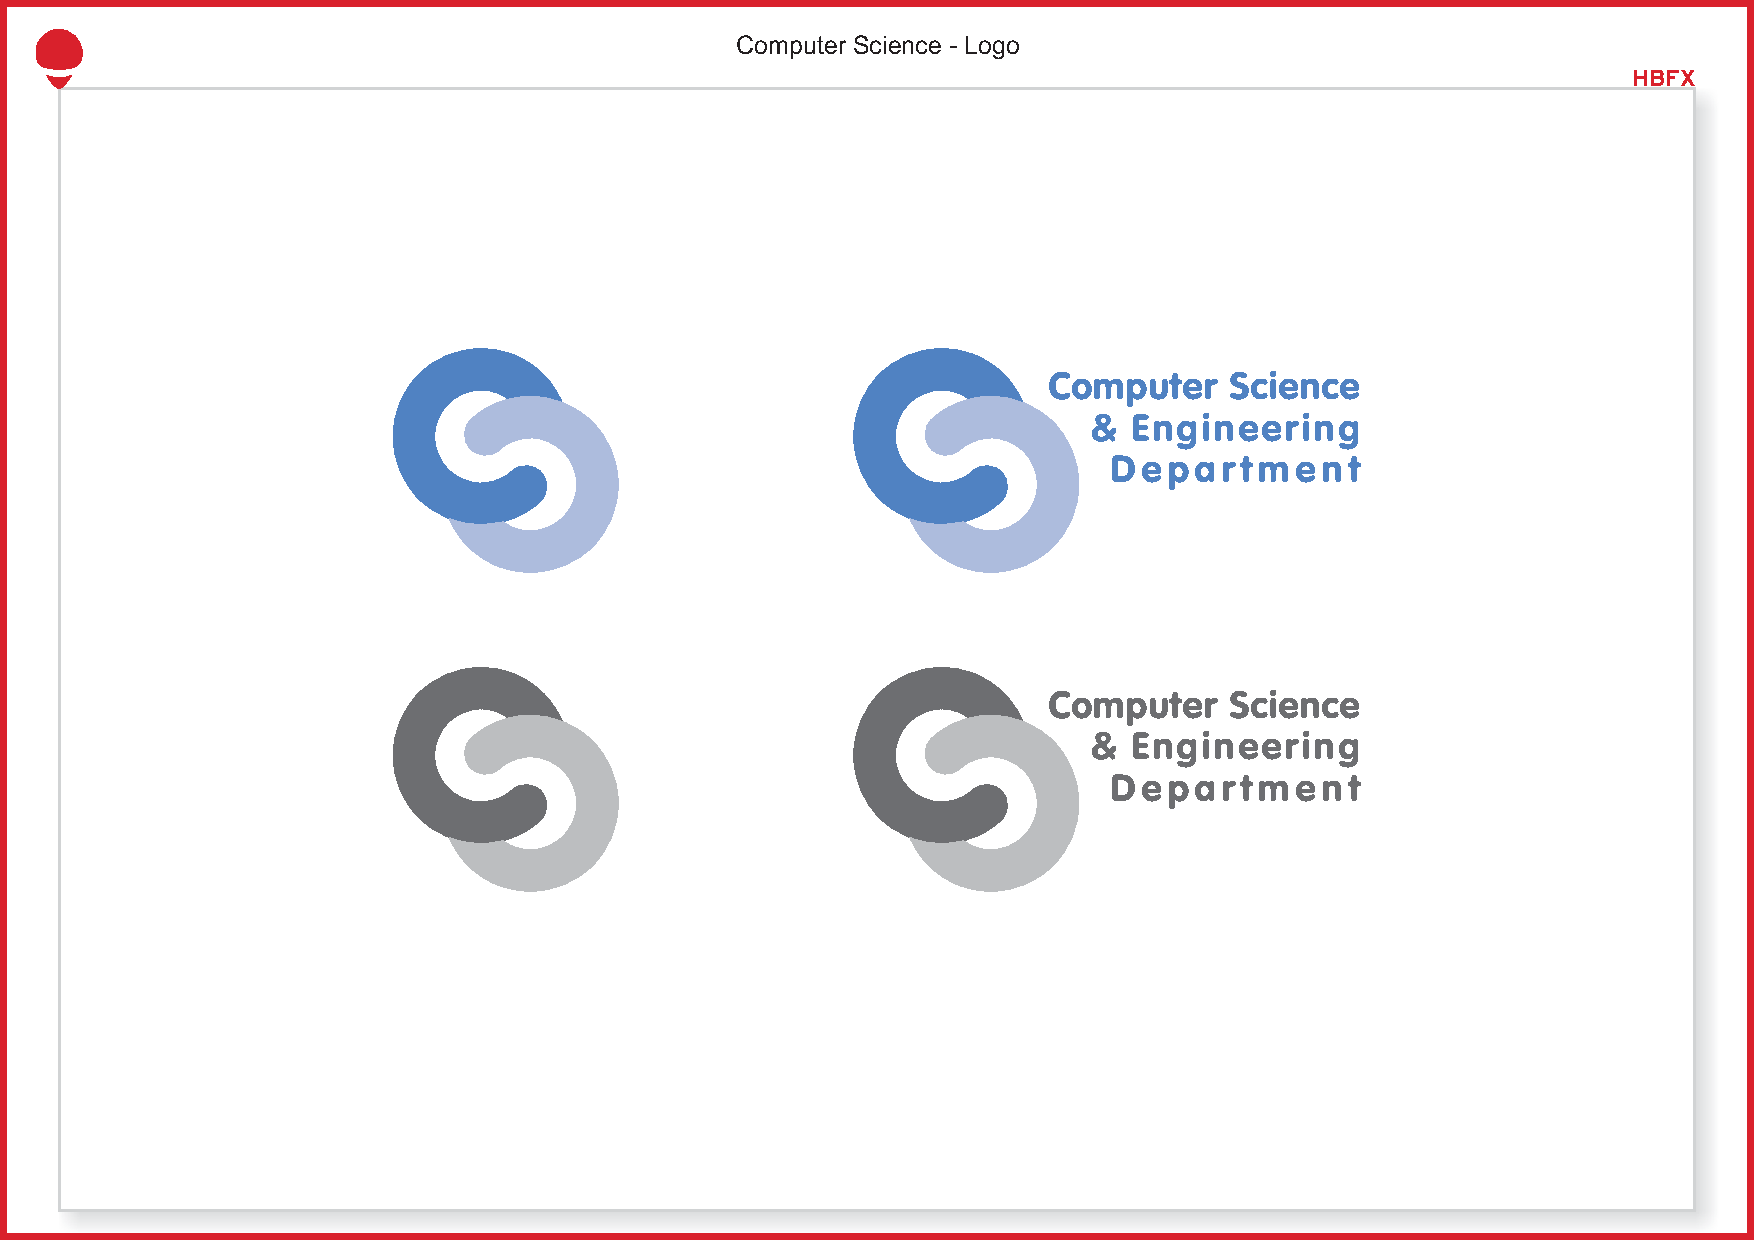
\includegraphics[scale=0.5,trim={14cm 11cm 2cm 5cm},clip=true]{pics/cs-logo.pdf}
\end{tabular}

\vspace{105pt}
{\Huge #2}\\                           % diploma project text
\vspace{40pt}
{\Large #3}\\ \vspace{0pt}  % project title
{\Large #4}\\                          % project subtitle
\vspace{40pt}
{\LARGE \Name}\\                   % student name
\end{center}
\vspace{60pt}
\begin{tabular*}{\textwidth}{@{\extracolsep{\fill}}p{6cm}r}
&{\large\textbf{#5}}\vspace{10pt}\\      % scientific advisor
&{\large \Advisor}                                    % advisor name
\end{tabular*}
\vspace{20pt}
\begin{center}
{\large\textbf{#6}}\\                                % bucharest
\vspace{0pt}
{\normalsize \Year}
\end{center}
\end{titlepage}
}

\newcommand{\frontPageEN}{\frontPage{\UniTextEN}{\DiplomaEN}{\ProjectTitleEN}{\ProjectSubtitleEN}{\AdvisorEN}{\BucEN}}

\linespread{1.15}
\setlength\parindent{0pt}
\setlength\parskip{.28cm}

%% Abstract macro
\newcommand{\AbstractPage}{
\begin{titlepage}
\textbf{\large ABSTRACT}\par
\AbstractEN \vfill
\end{titlepage}
}


%%%%%%%%%%%%%%%%%%%%%%%%%%%%%%%%%%%%%%%%%%%%%%%%%%   
%%
%%          End of template definitions
%%   
%%%%%%%%%%%%%%%%%%%%%%%%%%%%%%%%%%%%%%%%%%%%%%%%%%


%%% Puteți elimina aceste linii din lucrare, servesc numai pentru template.
\newcommand{\worktype}[1]{[\textit{#1}] }
\newcommand{\dezvoltare}{\worktype{Dezvoltare de produs}}
\newcommand{\cercetare}{\worktype{Cercetare}}
\newcommand{\ambele}{\worktype{Ambele}}
%%%


%%
%%   Campurile de mai jos trebuie modificate de autor. Modificati doar continutul, nu si numele fiecarei definitii
%%
\newcommand{\ProjectTitleEN}{Trading Bot}
\newcommand{\ProjectSubtitleEN}{Making an autonomous program that does the trading for you}
\newcommand{\Name}{Stanciu Stefan-Lucian}
\newcommand{\Advisor}{Prof. dr. ing. Radulescu Florin}
\newcommand{\Year}{2021}

% Setări document
\title{Proiect de diplomă}
\author{\Name}
\date{\Year}

%%
%%   Campurile aferente rezumatului
%%

\newcommand{\AbstractEN}{With the evolution of technology and with the apparition of the internet, in this day and age, purchasing and selling financial products has never been easier. In the past investors would call their broker to make a trade for them. They could either visit or telephone their broker, but now everything is being done on an online trading platform. Using these platforms can have a lot of benefits, but there is also one big downside, which is if you want to make money constantly then you have to be online for quite some time each day, in order to not miss some good deals. My application, MoneyTrading, aims to offer the customers of a trading platform, xStation from XTB, a tool that will automatically make transactions for them based on the their preferences.}


\begin{document}

\frontPageEN

\begingroup
\linespread{1}
\tableofcontents
\endgroup

\AbstractPage


\chapter{Introduction}\pagestyle{fancy}
\section{Context}
Traditionally, if investors or traders wanted to make a trade, they would have had to call their brokerage firms with a purchase or sell request. The process of confirming such an important request was a long and tedious one, with multiple phone calls or meetings in which a lot of topics needed to be addressed. The subjects that were approached by both parties involved (broker and the investor) were about the market's price, the limit price, how long to keep the order open for, in what account to purchase the shares (if the client had multiple accounts) and if the investment representative would approve the commission costs for making the trade. A lot of time and effort was spent on making transactions in the past.

Today, with so many advancements in the digital era, increasingly more investors are choosing to use online trading platforms from the comforts of their home, at any time they want. Online trading, simply put, refers to buying and selling financial assets using proprietary trading platforms offered by a broker for DIY (do-it-yourself) investing. As high-speed computers and good internet connections were made more and more accessible to every citizen, in the mid to late '90s the use of online trading increased exponentially. On such platforms there were made available, to purchase or sell, all kinds of currencies, stocks, bonds, options, funds, EFTs (electronic funds transfers). As of today, some of the most popular assets in the online trading domain are currencies, cryptocurrencies, stocks, commodities and one of the largest financial market in the world, larger even then the stock market, is the foreign exchange or forex, with an average daily trading volume of 6.6 trillion US dollars, according to the 2019 Triennial Central Bank Survey of FX and OTC derivatives markets \cite{centralBank}.

Nowadays, anyone can start trading online, simply, by opening a demat (dematerialized account that provides the facility of holding shares and securities in an electronic format) and creating an online account on a trading platform, but, in order to have success in this domain, it also requires a lot of information about the markets and about the stocks as stated in \cite{marketWizards}. There's quite a wealth of mostly free information out there on the internet like financial articles, stock market books and website tutorials from which one can grasp the intricacies of this domain. Online trading can be a really great way to earn a daily income as well as plan for the future, if it is done right.

\section{The Problem} 
The advent of online trading platforms, came with a lot of benefits, but also with some negatives, to both investors and traders. For example, one benefit is the improvement in speed and simplicity of which transactions can be made, due to the lack of need for paper-based documents to be copied, filed for each transaction. Another benefit is that an investor can now monitor the changes in market's prices and his investments all the time, but this benefit can also become one of the main disadvantages of online trading platforms, because it requires a lot of dedication and a lot of attention, in order to not lose money and make a profit. Online trading, can become a full time job for some investors, even if they already have another career, because of the need to be online on the platform for quite a while, day after day, monitoring each change in the market's price, making all the right transactions at the right moments, just to not lose out on potentially important or lucrative trades. In other words, online trading can consume a lot of time from a person's life, and that's the main problem that I'm trying to solve with this project.        
\section{Objectives}
The main goal of MoneyTrading, my application, is to address the main problem that was presented above. This tool will target the investors that are using xStation, the online trading platform from XTB, and it aims to make online trading a way of earning extra money without the need to constantly be online, avoiding the need to continuously stare at some price graphs, just waiting for the right opportunity to present itself, in order to make a good/profitable transaction and also, to change, for the better, the trading experience into a less time consuming, side or main, activity. To achieve the objectives stated above, my project will have to ease the transactions process by automatically overseeing any changes in prices from the markets and by performing purchase or sell orders based on the user's preferences and the current state of the market. 
\section{Proposed Solution} 
My application, MoneyTrading, features an user interface from which the consumer can login into their account on xStation, using their password and account number. After a successfully authentication, they can select on which markets to start making transactions and, most importantly, how and when to make the desired transactions. These user's choices are processed by an algorithm that determines, based on the conditions from the input, if a trade request needs to be made. Once the trading information is provided then it is sent to xStation platform using XTB's API.
\section{Obtained results}
The result is an autonomous program that does the trading for it's users. The transactions that it makes are entirely based on the user's input. It works on multiple markets at the same time, each market having it's own different options determined by the user. 
\section{Thesis Structure}
\begin{itemize}
	\item \textbf{Motivation and Requirements Analysis}: provides an insight into the motivation that made me develop my application, what it's functionalities are and what it's supposed to achieve
	\item \textbf{Related Work}: offers details about other products that have a similar purpose with my program and it also highlights some differences between the presented applications
	\item \textbf{Proposed Solution}: this chapter explores a detailed view of what technologies were used in the making of my project
	\item \textbf{Implementation Details}: provides an explanation of how the technologies from the previous chapter were used and how the algorithm works
	\item \textbf{Experimental Results}: presents the obtained results after using the application
	\item \textbf{Conclusion and Future Work}: this chapter gives an overview about what can be improved and what was gained from this project
\end{itemize}


\chapter{Motivation and Requirements Analysis}
\dezvoltare Acest capitol va analiza cerințele produsului din prisma potențialilor clienți și a scenariilor de utilizare preconizate, urmând a fi generată o lista de funcționalități. 

\cercetare Acest capitol va introduce motivația realizării proiectului propus.

Dacă proiectul de licență face parte dintr-un proiect mai amplu (de exemplu un proiect complex, la care lucrează 2 studenți (ex: 1 student la front-end-ul aplicației, 1 student la back-end-ul aplicației), în acest capitol va fi explicat pe scurt ansamblul proiectului și ce parte din proiect este adresată de lucrarea propusă. 

Criterii pentru calificativul \textit{Ne\textit{Satisfăcător}}: 
\begin{itemize}
	\item \dezvoltare Cerințele sunt imaginate de student pe baza unei analize a pieței;
	\item \cercetare Nu se oferă o motivație valida.
\end{itemize}

Criterii pentru calificativul \textit{Satisfăcător}: 
\begin{itemize}
	\item \dezvoltare Există un interviu, un client, analiza cerințelor este elaborată pe baza interviului;
	\item \cercetare Motivația este doar personala.
\end{itemize}


Criterii pentru calificativul \textit{Bine}: 
\begin{itemize}
	\item	 \dezvoltare Proces iterativ pe baza unor interviuri cu mai mulți clienți, dezvoltare MVP, reevaluare cerințe;
	\item	 \cercetare Motivația este legata de o necesitate științifica / tehnica explicită.
\end{itemize}


\chapter{Related Work}
\dezvoltare Ce soluții similare există pe piață? Care sunt limitările lor / pentru ce cazuri de utilizare sau pentru ce tip de clienți produsele existente pe piață nu răspund cerințelor? Care sunt indicatorii pe baza cărora sunt evaluate aceste produse, de către potențiali clienți, și unde sunt lipsurile/ care este oportunitatea generată de lipsurile acestea?

\cercetare Metode existente (sau ``State of the Art'') se referă, de regulă, la nivelul curent de dezvoltare: care este starea curentă a domeniului, unde ne găsim, care este contextul. Care sunt soluțiile actuale prezente în literatura de specialitate și care sunt limitările lor? Ce direcții de explorare sunt recomandate în literatura de specialitate? Literatura de specialitate se refera la articole științifice recente, publicate în reviste cu factor de impact mare, sau în volumele unor conferințe de top, sau în cărți.

\ambele În încheierea acestui capitol se dorește descrierea tehnologiilor folosite în lucrare, cu alternative și cu argumente convingătoare calitative și cantitative.  

Criterii pentru calificativul \textit{Ne\textit{Satisfăcător}}: 
\begin{itemize}
	\item \dezvoltare Sunt analizate superficial câteva produse de pe piață; 
	\item \cercetare analiza literaturii limitata la grupuri de cercetare din România;
	\item \ambele Sunt descrise tehnologiile folosite în lucrare. 
\end{itemize}

Criterii pentru calificativul \textit{Satisfăcător}:
\begin{itemize}
	\item \dezvoltare Există un interviu, un client, analiza cerințelor este elaborată pe baza interviului.
	\item \cercetare analiza literaturii de specialitate din lume, fără poziționarea precisă a lucrării în peisajului domeniului studiat;
	\item \ambele Sunt descrise câteva tehnologii alternative pentru fiecare din tehnologiile folosite în lucrare. Există o argumentare referitoare la alegere.
\end{itemize}

Criterii pentru calificativul \textit{Bine}:
\begin{itemize}
	\item \dezvoltare Proces iterativ pe baza unor interviuri cu mai mulți clienți, dezvoltare MVP, reevaluare cerințe;
	\item \cercetare analiza literaturii de specialitate din lume, cu poziționarea precisă a lucrării în peisajul actual al domeniului studiat; 
	\item \ambele Sunt descrise tehnologii alternative. Sunt analizate cantitativ și calitativ, folosite benchmarkuri și teste efectuate de student. Analiza este rezumată prin tabele și grafice.
\end{itemize}

\section{Similiar solutions}

Figurile utilizate în document vor fi centrate și numerotate (de exemplu Figura~\ref{fig:pic1}). 
Orice figură ce nu este realizată de către autorul lucrării va fi în mod obligatoriu citată fie la final (de exemplu Figura ~\ref{fig:pic2} este preluată din documentul \cite{}), fie cel puțin într-o notă de subsol (a se vedea Figura~\ref{fig:pic2}). Orice figură ce depășește ca dimensiune 50\% dintr-o pagină, va fi mutată la anexe. Toate figurile din cadrul tezei vor fi referite în text. Exemplu: Figura~\ref{fig:pic1} prezintă o schemă de principiu pentru un amplificator inversor cu AO. 

\begin{figure}[th]
\centering
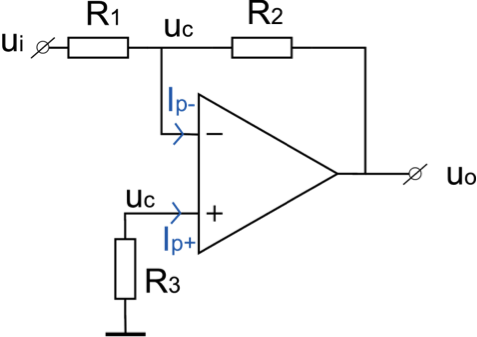
\includegraphics{pics/Pic1.png}
  \caption{Amplificator inversor}
  \label{fig:pic1}
\end{figure}

\newpage

\begin{figure}[th]
\centering
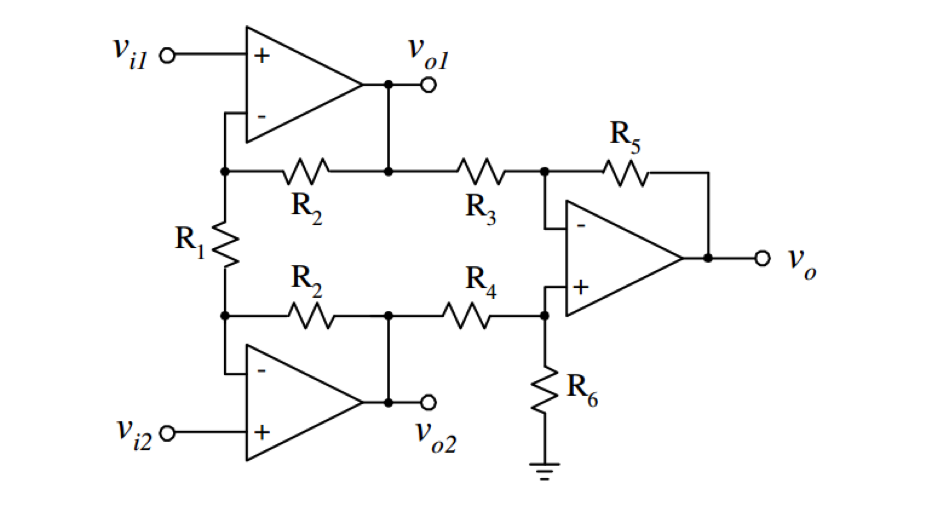
\includegraphics{pics/Pic2.png}
  \caption[Amplificator de instrumentație cu 3 AO-uri]{Amplificator de instrumentație cu 3 AO-uri\protect\footnotemark}
  \label{fig:pic2}
\end{figure}
\footnotetext{© http://www.ece.tamu.edu/sspalermo/ecen3205/Secton\%201III.pdf}

\chapter{Proposed Solution}
Capitolul conține o privire de ansamblu a soluției ce rezolvă problema, prin prezentarea structurii / arhitecturii acesteia. În funcție de tipul lucrării acest capitol poate conține diagrame (clase, distribuție, workflow, entitate-relație), demonstrații de corectitudine pentru algoritmii propuși de autor, abordări teoretice (modelare matematică), structura hardware, arhitectura aplicației.


Criterii pentru calificativul \textit{Ne\textit{Satisfăcător}}: 
\begin{itemize}
	\item	Descriere în limbaj natural.
\end{itemize}

Criterii pentru calificativul \textit{Satisfăcător}: 
\begin{itemize}
	\item	Descriere + diagrame de baze de date, workflow, clase, algoritmi. 
\end{itemize}

Criterii pentru calificativul \textit{Bine}: 
\begin{itemize}
	\item 	Descriere + diagrame de baze de date, workflow, clase, algoritmi + descrierea unui proces prin care s-a realizat arhitectura/structura soluției.
\end{itemize}

\section{Technologies}
Formulele matematice utilizate în document vor fi centrate în pagină și numerotate.

\begin{equation}
(x+a)^n = \sum_{k=0}^{n}\left(\begin{array}{c}n\\k\\\end{array}\right)x^ka^{n-k}
\end{equation}

\begin{equation}
f(x) = a_0 + \sum_{n=1}^{\infty}\left(a_n \cos\frac{n\pi x}{L} + b_n\sin\frac{n\pi x}{L}\right)
\end{equation}

\subsection{AWT API}

\subsection{Swing API}

\section{XTB Platform API}


\chapter{Implementation Details}
În plus fata de capitolul precedent acesta conține elemente specifice ale rezolvării problemei care au presupus dificultăți deosebite din punct de vedere tehnic. Pot fi incluse configurații, secvențe de cod, pseudo-cod, implementări ale unor algoritmi, analize ale unor date, scripturi de testare. De asemenea, poate fi detaliat modul în care au fost utilizate tehnologiile introduse in capitolul 3.


Criterii pentru calificativul \textit{Ne\textit{Satisfăcător}}: 
\begin{itemize}
	\item	Sunt prezentate pe scurt scheme și pseudo-cod.
\end{itemize}
Criterii pentru calificativul \textit{Satisfăcător}: 
\begin{itemize}
	\item	Descriere sumara a implementării, prezentarea unor secvențe nerelevante de cod, scheme, etc. 
\end{itemize}
Criterii pentru calificativul \textit{Bine}: 
\begin{itemize}
	\item	Descrierea detaliată a algoritmilor/structurilor utilizați; Prezentarea etapizată a dezvoltării, inclusiv cu dificultăți de implementare întâmpinate, soluții descoperite; (dacă este cazul) demonstrarea corectitudinii algoritmilor utilizați. 
\end{itemize}

\section{Using the XTB API}
Se recomandă utilizarea tabelelor de forma celui de mai jos.  Font size :  9. 
Orice tabel prezent în teză va fi referit în text; exemplu: a se vedea Tabel~\ref{tab:criterii}.

\section{Building the interface}

\section{The algorithm}

\subsection{Choosing the right design pattern}

\section{The optimisation}


\begin{table}[th]\small\linespread{1}
\caption{Sumarizare criterii}
\label{tab:criterii}
\begin{tabular}{l >{\raggedright\arraybackslash}p{8cm} >{\raggedright\arraybackslash}p{4cm}}
\textbf{Calificativ} & \textbf{Criteriu} & \textbf{Observații} \\\hline
\textbf{Nesatisfacator} & Sunt prezentate pe scurt scheme și pseudo-cod & \\\hline
\textbf{Satisfacator} &Descriere sumara a implementării, prezentarea unor secvențe nerelevante de cod, scheme, etc.& \\
\hline
\textbf{\textit{Bine}} &Descrierea detaliată a algoritmilor/structurilor utilizați; Prezentarea etapizată a dezvoltării, inclusiv cu dificultăți de implementare întâmpinate, soluții descoperite; (dacă este cazul) demonstrarea corectitudinii algoritmilor utilizați. & Pot fi incluse configurații, secvente de cod, pseudo-cod, implementări ale unor algoritmi, analize ale unor date, scripturi de testare. \\
\hline
\end{tabular}
\end{table}


\chapter{Experimental Results}
Acest capitol trebuie să răspundă, în principiu, la 2 întrebări și să se încheie cu o discuție a rezultatelor obținute. Cele doua întrebări la care trebuie sa se răspundă sunt:
\begin{enumerate}
	\item  \textbf{Merge corect?} (Conform specificațiilor extrase în capitolul 2); 
Evaluarea dacă merge corect se face pe baza cerințelor identificate în capitolele anterioare. 

	\item Cât de \textit{Bine} merge / cum se compară cu soluțiile existente? (pe baza unor metrici clare). 
Evaluarea cât de \textit{Bine} merge trebuie să fie bazată pe procente, timpi, cantitate, numere, \textbf{comparativ cu soluțiile prezentate în capitolul 3}. Poate fi vorba de performanță, overhead, resurse consumate, scalabilitate etc. 
\end{enumerate}

În realizarea discuției, se vor utiliza tabele cu procente, rezultate numerice și grafice. În mod obișnuit, aici se fac comparații și teste comparative cu alte proiecte similare (dacă există) și se extrag puncte tari și puncte slabe. Se ține cont de avantajele menționate și se demonstrează viabilitatea abordării / aplicației, de dorit prin comparație cu alte abordări (dacă acest lucru este posibil). Cuvântul cheie la evaluare este ``metrică'': trebuie să aveți noțiuni măsurabile și cuantificabile. În cadrul procesului de evaluare, explicați datele, tabelele și graficele pe care le prezentați și insistați pe relevanța lor, în următorul stil: ``este de preferat ... deoarece …''; explicați cititorului nu doar datele ci și semnificația lor și cum sunt acestea interpretate. Din această interpretare trebuie să rezulte poziționarea proiectului vostru printre alternativele existente, precum și cum poate fi acesta îmbunătățit în continuare.

Criterii pentru calificativul \textit{Ne\textit{Satisfăcător}}: 
\begin{itemize}
	\item Aplicația este testată dar rulează pe calculatorul studentului, nu există posibilități de testare, nu a fost validată cu clienți / utilizatori;
	\item Nu au fost realizate comparații cu alte sisteme similare.
\end{itemize}

Criterii pentru calificativul \textit{Satisfăcător}: 
\begin{itemize}
	\item \dezvoltare  Există teste unitare și de integrare, există o strategie de punere în funcțiune (deployment), există validare minimală cu clienții / utilizatorii.
	\item \cercetare Principalele componente și soluția în ansamblu au fost evaluate din punct de vedere al performanței, însă nu sunt folosite seturi de date standard, există unele erori de interpretare a datelor.
	\item \ambele Discuție minimală asupra relevanței rezultatelor prezentate, comparație minimală cu alte sisteme similare.
\end{itemize}

Criterii pentru calificativul \textit{Bine}: 
\begin{itemize}
	\item \dezvoltare Teste unitare și de integrare, instrumente de punere in funcțiune (deployment) utilizate și care arată lucru constant de-a lungul semestrului, lucrare validată cu clienții / utilizatorii, produs în producție.
	\item \cercetare Componentele și soluția în ansamblu au fost evaluate din punct de vedere al performanței, folosind seturi de date standard și cu o interpretare corectă a rezultatelor.
	\item \ambele Discuție cu prezentarea calitativă și cantitativă a rezultatelor, precum și a relevanței acestor rezultate printr-o comparație complexă cu alte sisteme similare.
\end{itemize}

\chapter{Conclusion and Future Work}
În acest capitol este sumarizat întreg proiectul, de la obiective, la implementare, si la relevanta rezultatelor obținute. În finalul capitolului poate exista o subsecțiune de ``Dezvoltări ulterioare''.

Criterii pentru calificativul \textit{Ne\textit{Satisfăcător}}: 
\begin{itemize}
	\item	Concluziile nu sunt corelate cu conținutul lucrării;
\end{itemize}

Criterii pentru calificativul \textit{Satisfăcător}: 
\begin{itemize}
	\item	Concluziile sunt corelate cu conținutul lucrării, însă nu se oferă o imagine asupra calității și relevantei rezultatelor obținute;
\end{itemize}

Criterii pentru calificativul \textit{Bine}: 
\begin{itemize}
	\item	Concluziile sunt corelate cu conținutul lucrării, și se oferă o imagine precisa asupra relevantei și calității rezultatelor obținute în cadrul proiectului. 
\end{itemize}

\chapter*{Bibliography}\addcontentsline{toc}{chapter}{Bibliography}  
% * <marios.choudary@gmail.com> 2018-02-28T12:07:48.730Z:
% 
% > BIBLIOGRAFIE
% Am adaugat un paragraf cu cateva detalii despre folosirea citarilor bibliografice in Latex, despre folosirea lui "\cite" si despre posibilitatea folosirii bibliografiei si direct in fisierul Latex.
% 
% ^.

\begin{itemize}
	\item 	NU utilizați referințe la Wikipedia sau alte surse fără autor asumat.
	\item 	Pentru referințe la articole relevante accesibile în web (descrise prin URL) se va nota la bibliografie și data accesării.
	\item 	Mai multe detalii despre citarea referințelor din internet se pot regăsi la:
	\begin{itemize}
		\item	\url{http://www.writinghelp-central.com/apa-citation-internet.html}
		\item	\url{http://www.webliminal.com/search/search-web13.html}
	\end{itemize}
	\item 	Note de subsol se utilizează dacă referiți un link mai puțin semnificativ o singură dată; Dacă nota este citată de mai multe ori, atunci utilizați o referință bibliografică.
	\item 	Dacă o imagine este introdusă în text și nu este realizată de către autorul lucrării, trebuie citată sursa ei (ca notă de subsol sau referință - este de preferat utilizarea unei note de subsol).
	\item 	Referințele se pun direct legate de text (de exemplu ``KVM [1] uses'', ``as stated by Popescu and Ionescu [12]'', etc.). Nu este recomandat să folosiți formulări de tipul ``[1] uses'', ``as stated in [12]'', ``as described in [11]'' etc..
	\item 	Afirmațiile de forma ``are numerous'', ``have grown exponentially'', ``are among the most used'', ``are an important topic'' trebuie să fie acoperite cu citări, date concrete si analize comparative.
	\begin{itemize}
		\item	Mai ales în capitolele de introducere, ``state of the art'', ``related work'' sau ``background'' trebuie să vă argumentați afirmațiile prin citări. Fiți autocritici și gândiți-vă dacă afirmațiile au nevoie de citări, chiar și cele pe care le considerați evidente.
		\item	Cea mai mare parte dintre citări vor fi în capitolele de introducere ``state of the art'', ``related work'' sau ``background''.
	\end{itemize}
	\item 	Toate intrările bibliografice trebuie citate în text. Nu le adăugați pur și simplu la final.
	\item 	Nu copiați sau traduceți niciodată din surse de informație de orice tip (online, offline, cărți, etc.). Dacă totuși doriți să oferiți, prin excepție, un citat celebru - de maxim 1 frază- utilizați ghilimele și evident menționați sursa. .
	\item 	Dacă reformulați idei sau creați un paragraf rezumat al unor idei folosind cuvintele voastre, precizați cu citare (referință bibliografică) sau cu notă de subsol sursa sau sursele de unde ați preluat ideile.
\end{itemize}

Trebuie respectat un singur standard de trimiteri bibliografice (citare), dintre următoarele alternative:
\begin{itemize}
	\item APA (\url{http://pitt.libguides.com/c.php?g=12108\&p=64730})
	\item IEEE (\url{https://ieee-dataport.org/sites/default/files/analysis/27/IEEE\%20Citation\%20Guidelines.pdf}) 
	\item Harvard (\url{https://libweb.anglia.ac.uk/referencing/harvard.htm})
	\item Cu numerotarea referințelor în ordine alfabetică sau în ordinea apariției în text (de exemplu, stilul cu numere folosit de unele publicații ACM - \url{https://www.acm.org/publications/authors/reference-formatting}) 
\end{itemize}

În Latex este foarte ușor să folosiți referințe într-un mod corect și unitar, fie prin adăugarea unei secțiuni
\verb!\begin{thebibliography}!
(vezi la sfârșitul acestei secțiuni), fie printr-un fișier separat de tip bib, folosind comanda
\verb!\bibliography{}!,
așa cum procedăm mai jos prin folosirea fișierului ``bibliography.bib''. În orice caz, în Latex va trebui să folosiți comanda
\verb!\cite{}!
pentru a adăuga referințe, iar această comandă trebuie folosită direct în text, acolo unde vreți sa apară citația, ca în exemplele următoare:

\textbf{Important}: în această secțiune de obicei apar doar intrările bibliografice (adică doar listarea referințelor). Citarea lor prin comanda cite și explicații legate de ele trebuie facute în secțiunile anterioare. Citarea de mai sus a fost facută aici doar pentru exemplificare.

% Asa se specifica folosirea unui fisier cu referinte bibliografice:
\bibliographystyle{plain}
\bibliography{bibliography}

%% O alta varianta ar fi fost includerea de articole direct in acest fisier
%% in felul urmator:
%% \begin{thebibliography}{ABC}
%%
%% \bibitem{article}
%%  H. Baali, H. Djelouat, A. Amira and F. Bensaali,
%%  ``Empowering Technology Enabled Care Using IoT and Smart Devices:
%   A Review''. In: IEEE Sensors Journal, vol. 322 (10), pp. 891--921, 1905.
%%
%% (more \bibitem items here...)
%%
%% \end{thebibliography}

%% Daca vreti ca o sectiune sa inceapa pe o pagina noua, puteti forta acest lucru cu comanda "\newpage", ca mai jos:

%\newpage

\end{document}